\section{Trattazione degli errori}\label{sez_errori}
\subsection{Conteggi}\label{sez_err_conteggi}
Per la determinazione dell'errore sui conteggi, abbiamo utilizzato la radice quadrata dei conteggi stessi, in accordo con la statistica di Poisson. Pertanto, per l'errore associato al numero di conteggi, ovvero per $\sigma_{N_{s}}$, abbiamo preso $\sqrt{N_{S}}$ mentre per $\sigma_{N_{i}}$ abbiamo preso $\sqrt{N_{i}}$. Oltre a questo è importante prestare attenzione ad un errore sistematico presente in ogni misura legato alla scelta dell'intervallo di integrazione dello spettro.

Il termine $N_s/N_i$ che compare all'iterno della formula della sezio d'urto differenziale (\ref{eq sezione d'urto conteggi}) è composta da due misure correlate tra di loro di conseguenza trattandola come una binomiale si ottiene che l'errore su questo rapporto è:
\begin{equation}
    \sigma_{\frac{N_s}{N_i}}=\frac{1}{N_i}\sqrt{N_s\left(1-\frac{N_s}{N_i}\right)}
\end{equation}
\subsection{Angolo solido}\label{sez_err_angolo_solido}
Per quanto riguarda la misura dell'angolo solido l'errore è stato inizialmente calcolato tramite propagazione della relazione geometrica introdotta in eq. \eqref{eq:angolo_solido} e rappresentata in fig. \ref{fig:angolo_solido}. Introducendo le grandezze geometriche da noi misurate si ottiene:
\begin{equation}
    \Delta\Omega = \frac{\pi (d/2)^2}{l^2 + (d/2)^2}
\end{equation}
\begin{figure}[H]
    \centering
    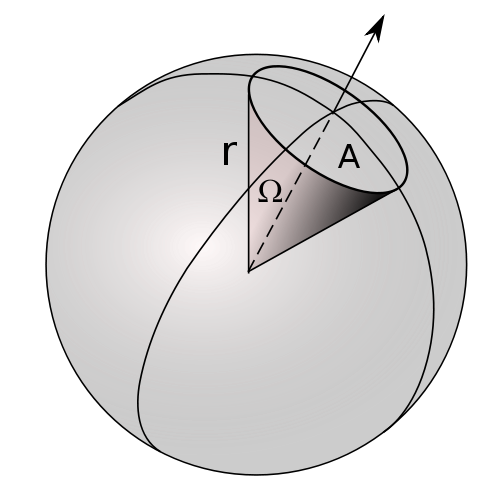
\includegraphics[scale=0.2]{Errori/solid_angle.png}
    \caption{Rappresentazione geometrica dell'angolo solido sotteso}
    \label{fig:angolo_solido}
\end{figure}
Nel nostro caso il termine $d$ è il diametro del rivelatore A , mentre $l$ è la distanza bersaglio-rivelatore A. La propagazione degli errori ha dunque prodotto la seguente espressione:
\begin{equation}
    \sigma_{\Delta\Omega} = \frac{8\pi d l}{(4l^2+d^2)^2} \sqrt{l^2 \sigma_{d}^2 + d^2 \sigma_{l}^2}
    \label{eq:err_angolo_solido}
\end{equation}
Per quanto riguarda $\sigma_d$ si è ritenuto ragionevole utilizzare l'errore strumentale del calibro ($\pm0.05\unit{\cm}$) con il quale si è misurato il diametro del rivelatore.\\La distanza bersaglio-rivelatore veniva invece misurata con il metro ed è certamente la misura con maggior contributo di errore.\\
Poichè il contributo di errore dovuto all'angolo solido è quello di maggior peso, come confermato dalla simulazione Montecarlo in sezione \ref{sezione d'urto e montecarlo}, si sono fatte alcune considerazioni in merito. Dopo alcune riflessioni si è infatti considerato che ad ogni dato angolo di misura la distanza $l$ dipende in realtá dal punto in cui interagisce il fotone con il bersaglio; motivo per cui l'errore associato é stato stimato a $\sigma_l = \pm 1 \unit{\cm}$. Questo perché considerando le ipotesi peggiori, cioé che lo scattering avvenisse sul bordo del bersaglio, la distanza $l$ effettiva si distacca in media (nelle varie configurazioni angolari) di circa $\pm 1 \unit{\cm}$ dal valore misurato di $14.4\unit{cm}$ .\\Queste riflessioni ci hanno dunque spinto ad aumentare l'errore rispetto a quello strumentale; tuttavia permettono solamente una stima qualitativa. In prospettiva sarebbe stato meglio scegliere una geometria tale da aumentare le distanze, e di conseguenza diminuire gli angoli solidi coperti, migliorando cosí l'errore percentuale sulla distanza $l$ a discapito di un minor rate di conteggi al secondo.
\subsection{Sezio d'urto e Simulazione Montecarlo}\label{sezione d'urto e montecarlo}
Per valutare l'errore associato alla misura della sezione d'urto è stata utilizzata la teoria della propagazione degli errori ottenendo la seguente fotmula:
\begin{equation}
    \sigma_{\frac{d\sigma}{d\Omega}} = \frac{M}{\Delta\Omega N_{A} \rho dx} \sqrt{\frac{N_{S}^{2}}{N_{i}^{2} \Delta\Omega^{2}} \sigma_{\Delta\Omega}^{2}+\sigma_{\frac{N_{S}}{N_{i}}}^{2}+\frac{N_{S}^{2}}{N_{i}^{2} dx^{2}}\sigma^2_{dx}}
\end{equation}
Al fine di completare l'analisi degli errori sperimentali associati alla misura della sezione d'urto dell'effetto Compton, è stata sviluppata e implementata una simulazione Montecarlo. Questo approccio è stato adottato con l'obiettivo di verificare l'accuratezza delle formule utilizzate per la propagazione degli errori e per identificare quali parametri sperimentali contribuiscano maggiormente all'incertezza complessiva della misura. Il codice utilizzato per la simulazione è reso disponibile nella repository di github\footnote{Codice consultabile al seguente link: \url{https://gitfront.io/r/MicheleScattola/GaGvFGBPX4Vm/Misure-Nucleari/tree/Compton/Montecarlo/}}. Dall'analisi dei risultati grafici ottenuti, presentati nelle Figure (\ref{fig:Simulazione_misura}) e (\ref{fig:simulazione_errori}) emerge che la propagazione degli errori è consistente con le previsioni teoriche. In particolare, è possibile constatare che il principale contributo all'incertezza nella misura della sezione d'urto è attribuibile alla misura dell'angolo solido.
\begin{figure}[H]
  \centering
  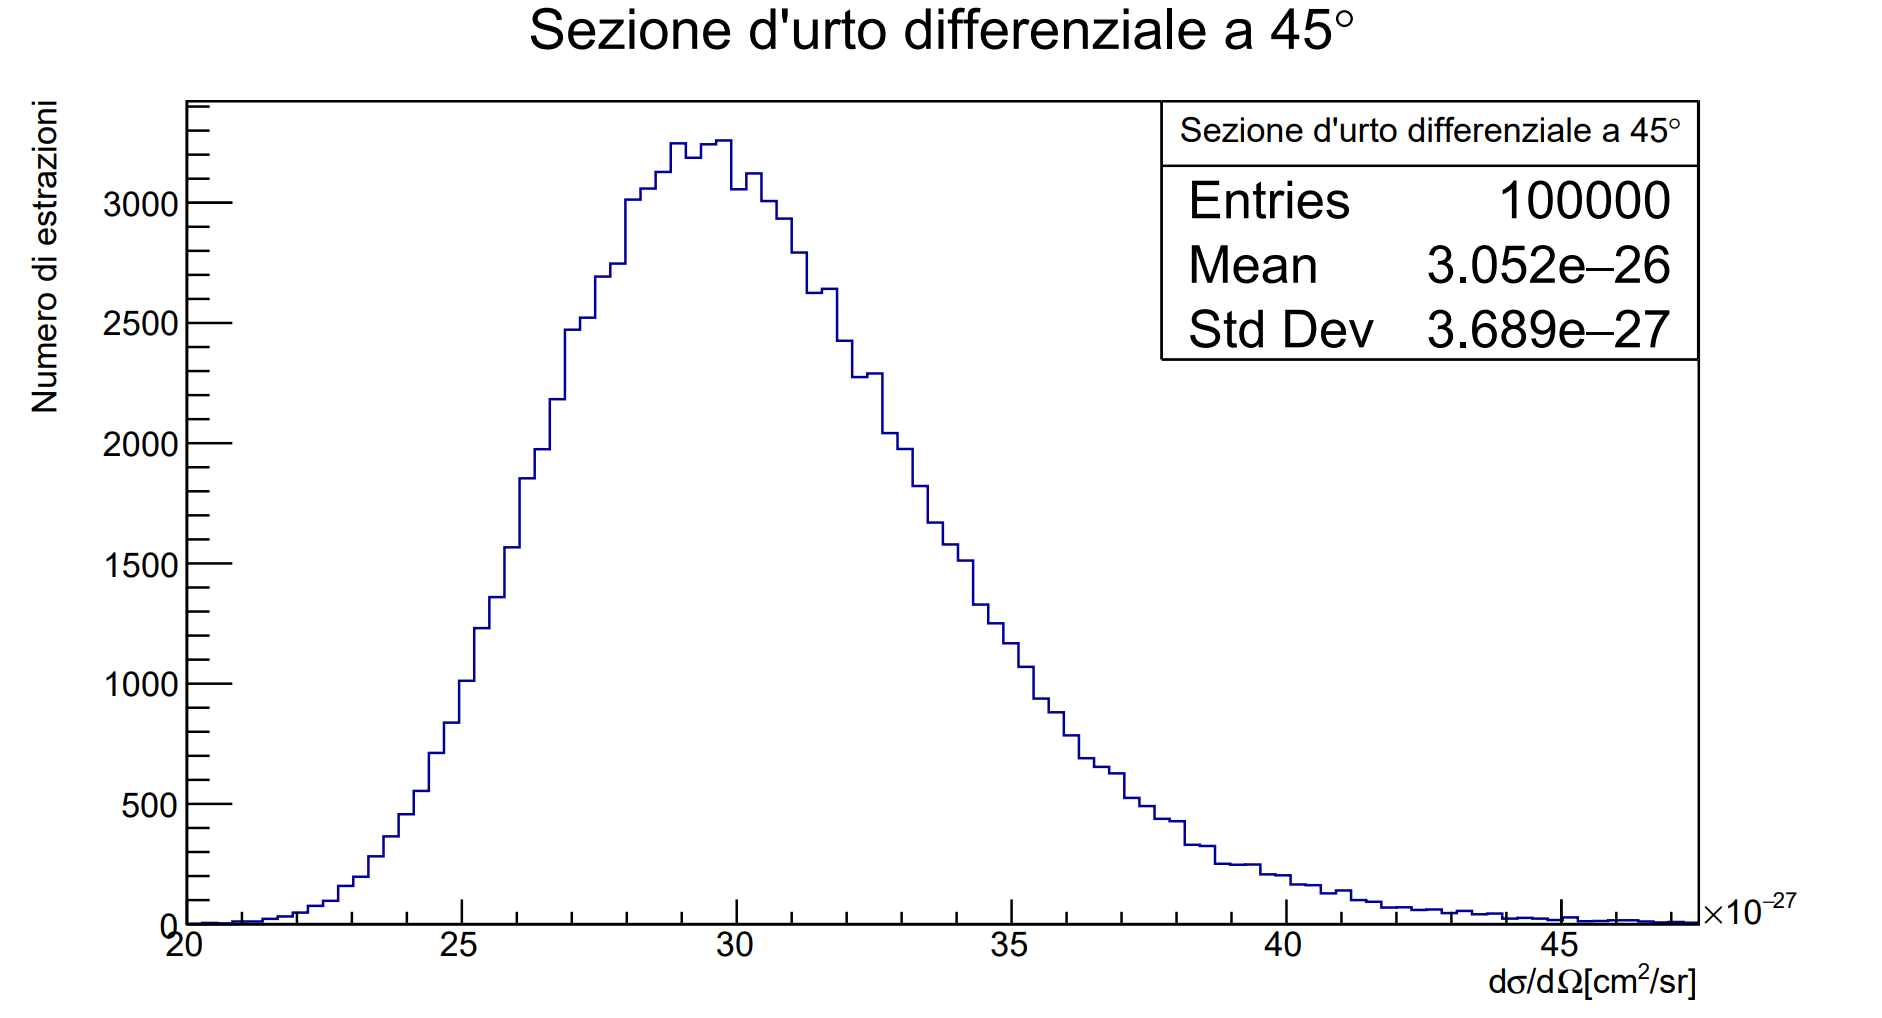
\includegraphics[scale=0.25]{Analisi Dati/SimulazioneMontecarlo_misura.png} 
  \caption{Simulazione di 100,000 misure della sezione d'urto Compton}
  \label{fig:Simulazione_misura}
\end{figure}
\begin{figure}[H]
  \centering
  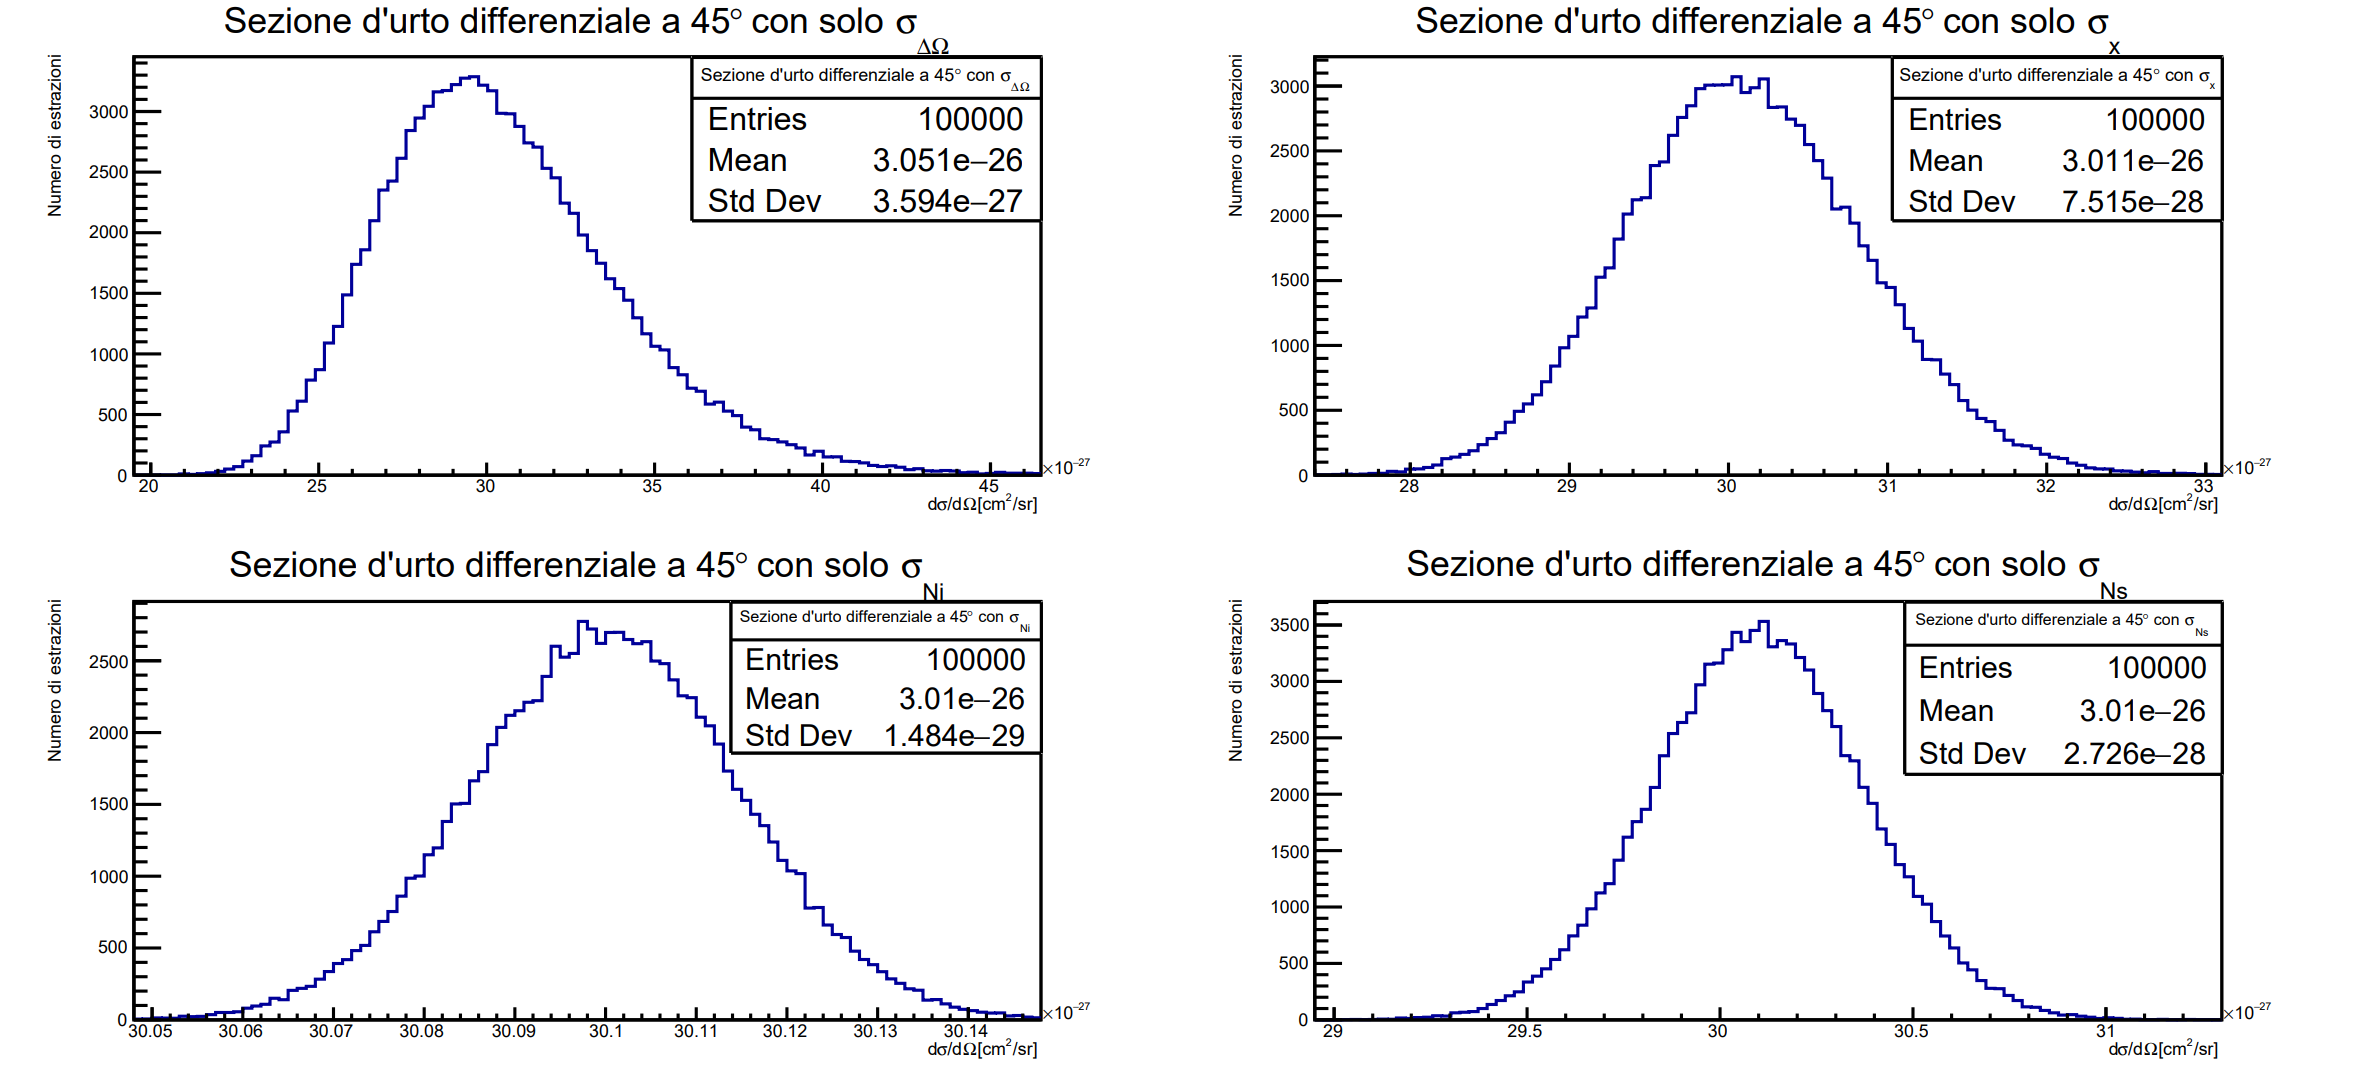
\includegraphics[scale=0.3]{Analisi Dati/SimulazioneMontecarlo_errori.png} 
  \caption{Simulazione di 100,000 misure della sezione d'urto Compton, con l'isolamento sequenziale degli errori sperimentali.}
  \label{fig:simulazione_errori}
\end{figure}
